\documentclass{ctexart}

\usepackage{graphicx}
\usepackage{amsmath}
\usepackage{float}

\title{Programming 4}

\author{洪晨瀚 \\ 信息与计算科学 3200300133}

\begin{document}

\maketitle
\graphicspath{{image/}}



\section*{Question A}
\begin{flushleft}
  \begin{figure}[H]
  \centering
    \centering
    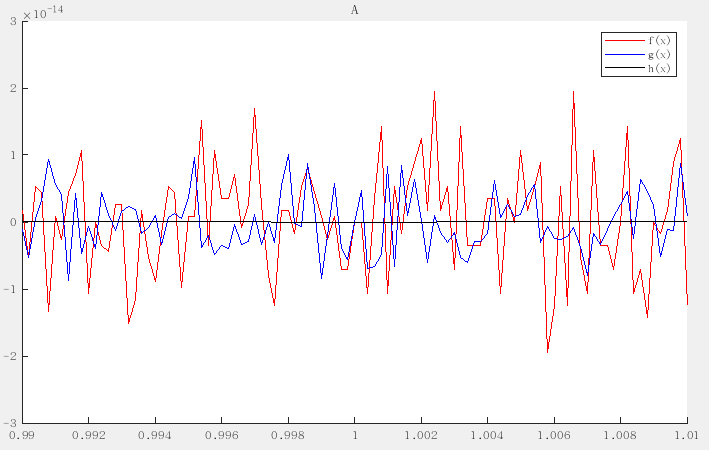
\includegraphics[width=12cm]{A}
    \caption{A}
  \end{figure}
  
  We see that f(x) and g(x) are wild fluctuation and h(x) is most accurate, it is because h(x) only have once subtraction and none addition but f(x) and g(x) have many.
\end{flushleft} 

\clearpage

\section*{Question B}
\begin{flushleft}
  (1)\\
  UFL : 0.5\\
  OFL : 3.5\\

  (2)\\
  All normal numbers of F : \\
  -3.5 , -3 , -2.5 , -2 , -1.75 , -1.5 , -1.25 , -1 , -0.875 , -0.75 , -0.625 , -0.5 , 0 , 0.5 , 0.625 , 0.75 , 0.875 , 1 , 1.25 , 1.5 , 1.75 , 2 , 2.5 , 3 , 3.5

  
  (3)\\
  \begin{figure}[H]
  \centering
    \centering
    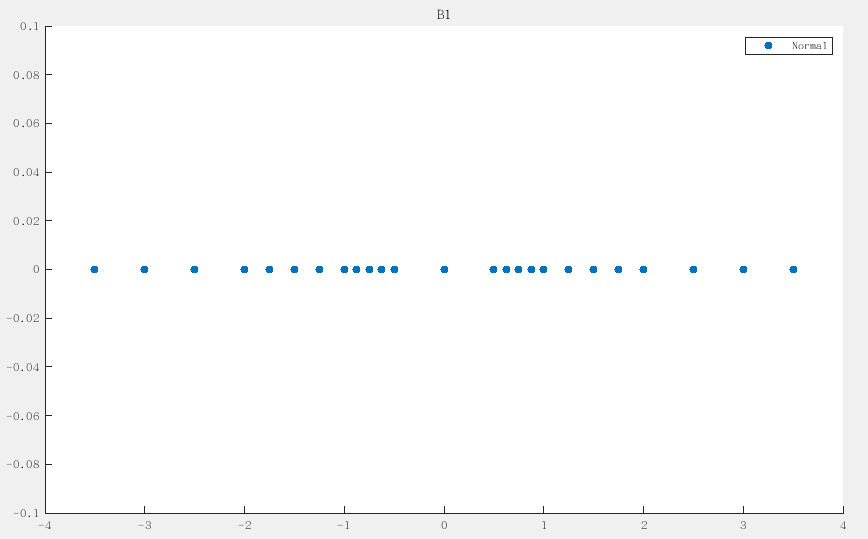
\includegraphics[width=12cm]{B1}
    \caption{B1}
  \end{figure}

  \clearpage
  
  (4)\\
  All subnormal numbers of F : \\
  -0.1875 , -0.125 , -0.0625 , 0.0625 , 0.125 , 0.1875

  (5)\\
  \begin{figure}[H]
  \centering
    \centering
    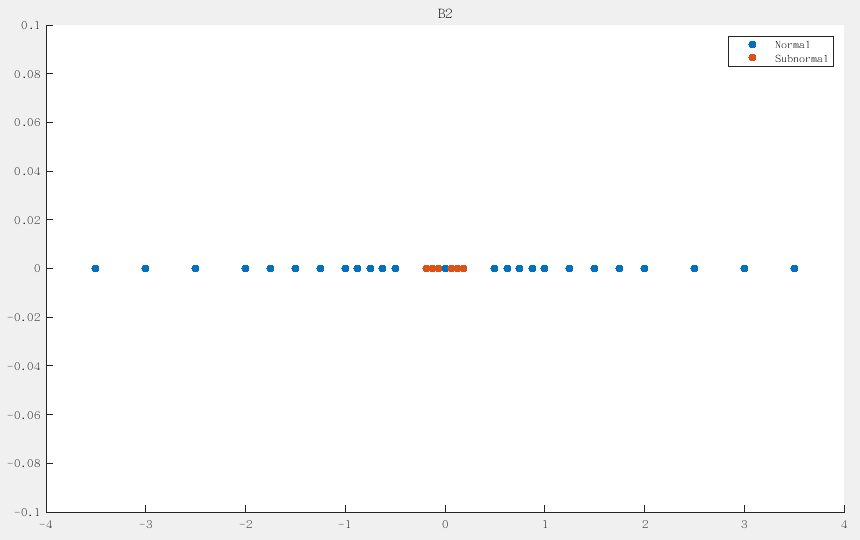
\includegraphics[width=12cm]{B2}
    \caption{B2}
  \end{figure}
\end{flushleft}

\end{document}
